% !TeX root = Ausarbeitung_Anna-Lena_Marx.tex


%Laden des Datensatzes
%Exploration, Zusammenfassung und Visualisierung des Datensatzes
%Entwurf, Training und Test mehrer Modellarchitekturen
%Nutzung der Modelle, um Vorhersagen für neue Bilder zu treffen, und die Prognosegüte zu ermitteln.
%Zusammenfassung der Ergebnisse mit einem schriftlichen Bericht


\section{Maschinelles Lernen von belgischen Verkehrszeichen}
Diese Arbeit basiert auf dem belgischen Verkehrszeichen Datensatz (Belgian Traffic Sign Dataset) \cite{Timofte-MVA-2011}, der zum Training und zur Validierung des Modells genutzt werden soll. 
Der Datensatz für Training und Testing ist frei unter \url{https://btsd.ethz.ch/shareddata/BelgiumTSC/} verfügbar. \\
\\
Der Datensatz beeinhaltet Verkehrszeichen aus 62 Kategorien. Es handelt sich dabei also um eine Klassifikationsaufgabe, bei der jeweils ein einzelnes Bild eines Verkehrszeichen richtig zugeordnet werden soll. 
Im Rahmen dieser Hausarbeit sollen mit Hilfe des Frameworks \textit{Keras} mehrere Modelle von neuronalen Netzen entwickelt, mit dem Trainingsdatensatz trainiert und abschließend anhand ihrer Leistung aber auch der Architektur verglichen und bewertet werden. Abschließend soll die Leistungsfähigkeit der Modelle durch Bilder, die nicht dem Trainings- oder Testdatensatz angehören überprüft werden.

\section{Keras}
Keras wird als High-Level API für neuronale Netze beschrieben, die eine sehr einfache und schnelle Entwicklung dieser zum Ziel hat \cite{keras}. Das Framework selbst ist in Python geschrieben und nutzt TensorFlow \footnote{\url{https://www.tensorflow.org/}} (Google), CNTK \footnote{\url{https://github.com/Microsoft/cntk}} (Microsoft) oder Theano \footnote{\url{https://github.com/Theano/Theano}} (MILA, eingestellt) als Backend-Bibliothek für die eigentlichen Berechnungen. Keras selbst ist eine eigenständige Bibliothek und wird als solche entwickelt, gehört aber seit dem Release von TensorFlow 1.4 zur TensorFlow Core API. 
Wie auch TensorFlow ist Keras Open-Source und auf GitHub einsehbar.
Innerhalb dieser Arbeit wird Keras in der Version 2.2.2 mit TensorFlow 1.9.0 als Backend auf einer Linux-Plattform genutzt. \\
\\
Die Wahl von Keras als Framework ist durch die Klarheit und Verständlichkeit der API begründet. Dennoch steht mit TensorFlow eine bekannte, gut getestete und sehr mächtige Implementierung für maschinelles Lernen zur Verfügung. 
Für die Entwicklung und das Training wurde eine Intel(R) Core(TM) i7-7820HQ CPU mit 8 virtualisierten Kernen und 16 GB RAM verwendet. Auf eine für den Befehlssatz der CPU oder eine GPU optimierte Implementierung von TensorFlow wurde dabei verzichtet.

\section{Der Datensatz}
Der belgische Verkehrszeichen Datensatz unterscheidet zwischen 62 verschiedenen, aber teils sehr ähnlichen Kategorien. In den Abbildungen \ref{pic:vergleich-zeichen1} und \ref{pic:vergleich-zeichen2} ist dies anhand von Originalbildern aus den Trainingsdaten dargestellt. Während Bild (a) aus der Abbildung \ref{pic:vergleich-zeichen1} zwar Ähnlichkeiten mit den anderen beiden aufweist, ist es durch die Form klar abzugrenzen. Zwischen den Bildern (b) und (c) ist dies deutlich schwieriger. Bei Bild (b) handelt es sich um ein Gefahrenzeichen, während (c) ein rein informativen Charakter hat \cite{road-sign-defs}. Der Unterschied in Farbe und Form ist, gerade bei der Nutzung von Bildern in Graustufen nicht sehr groß. In der Anwendung einer künstlichen Intelligenz im Straßenverkehr ist die korrekte Unterscheidung zwischen Information und Gefahrenzeichen durchaus relevant. 
Noch deutlicher wird die Schwierigkeit in der Klassifikation in den unter Abbildung \ref{pic:vergleich-zeichen2} dargestellten Originalbildern. Es handelt sich tatsächlich um das selbe Zeichen, dass durch seine Ausrichtung eine gewisse Bedeutung erlangt. Der Datensatz unterscheidet zwischen \textit{mandatory direction (ahead)} (a) und \textit{mandatory direction (others)} (b und c). 
Damit ist die Klassifikation in diesem Fall von der Ausrichtung der Eingangsbilder abhängig. Schon bei einer leichten Verzerrung ist es denkbar, dass ein Modell zur Klassifikation die falsche Klasse auswählt. Dies wäre in der realen Welt aber auch bei einem menschlichen Fahrer leicht möglich, zeigt aber gut eine Schwierigkeit die aus dem Datensatz selbst resultiert.

\begin{figure} [ht]
	\centering
	\subfloat[][]{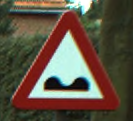
\includegraphics[width=0.2\linewidth]{0}}%
	\qquad
	\subfloat[][]{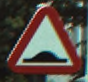
\includegraphics[width=0.2\linewidth]{1}}%
	\qquad
	\subfloat[][]{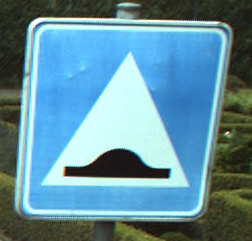
\includegraphics[width=0.2\linewidth]{59}}%
	\caption{(a) Klasse 0 \textit{Uneven road}, (b) Klasse 1 \textit{speed bump} , (c) Klasse 59 \textit{speed bump}}%
	\label{pic:vergleich-zeichen1}
\end{figure}

\begin{figure} [ht]
	\centering
	\subfloat[][]{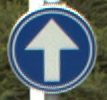
\includegraphics[width=0.2\linewidth]{34}}%
	\qquad
	\subfloat[][]{
\includegraphics[width=0.2\linewidth]{35}}%
	\qquad
	\subfloat[][]{
\includegraphics[width=0.2\linewidth]{35-2}}%
	\caption{(a) Klasse 34 \textit{mandatory direction (ahead)}, (b) Klasse 35 \textit{mandatory direction (others)} , (c) Klasse 35 \textit{mandatory direction (others)}}%
	\label{pic:vergleich-zeichen2}
\end{figure} \ \\
%
Eine andere solche Schwierigkeit ist die Größe und Aufteilung des Datensatzes. Auf der schon genannten Website kann jeweils ein Trainings- und ein Testdatensatz heruntergeladen werden. Ein klar abgegrenzter Datensatz zur Validierung ist nicht verfügbar. Durch die Größe von Trainings- und Testdatensatz mit 4570 bzw. 2520 Bildern aufgeteilt sehr gering ist, kann nicht ohne weiteres ein Validierungsdatensatz abgetrennt werden. Auch die Aufteilung der Bilder im größeren Trainingsdatensatz erschwert dies. Abbildung \ref{pic:picsproclass} stellt die Problematik dabei gut dar. Während für 16 Klassen mindestens 100 Beispielbilder, anhand derer das neuronale Netz trainiert werden kann, vorhanden sind, müssen für 5 Klassen unter 10 Beispielbilder genügen. Machine Learning Verfahren leben von einer möglichst großen Datenmenge für das Training, es ist daher anzunehmen, dass für die 5 Klassen mit weniger als 10 Beispielbilder schlechtere Vorhersage-Ergebnisse als für die 16 Klassen mit mehr als 100 Beispielbildern erzielt werden. Zudem ist es auch hierdurch äußerst schwierig und wenig zielführend ein weiteren, distinkten Datensatz zur Verifikation abzugrenzen. 

\begin{figure} [ht]
	\centering
	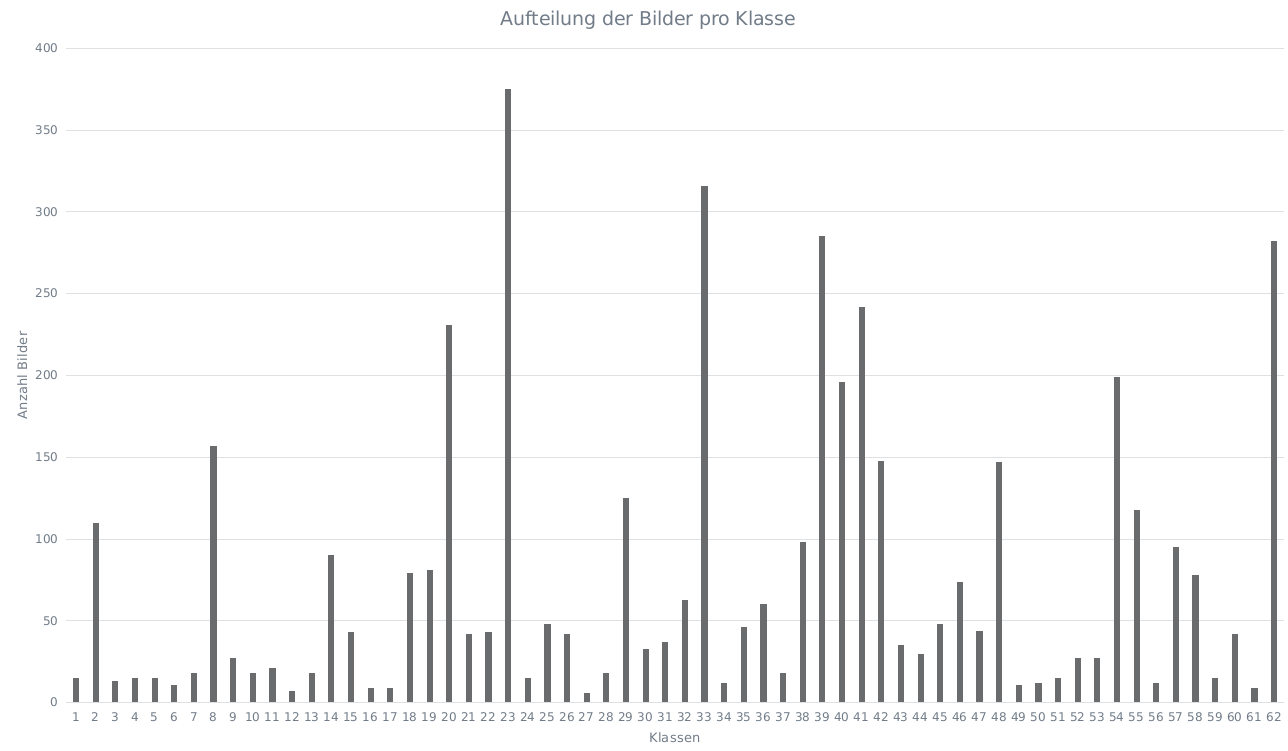
\includegraphics[width=\linewidth]{BilderProKlasse}
	\caption{Verteilung der Bilder pro Klasse für den Trainingsdatensatz}
	\label{pic:picsproclass}
\end{figure} \ \\
%
In den Abbildungen \ref{pic:vergleich-zeichen1} und \ref{pic:vergleich-zeichen2} werden bereits Beispielbilder aus dem Trainingsdatensatz dargestellt. Die Bilder liegen als Farbbilder (RGB) im PPM (Portable Pixmap) Format, aber in unterschiedlichen Bildgrößen vor. Die Bilder sind für Trainings- und Testdatensatz jeweils in Unterordnern, welche die Klassen repräsentieren, angeordnet. Zusätzlich befindet sich in jedem Unterordner eine CSV-Datei, die zusätzliche Informationen, wie die Breite, die Höhe, die Koordinaten der Region of Interest (ROI) und die Klassennummer, zu jedem Bildnamen enthält. Die Informationen aus dieser Datei wurden in dieser Arbeit nicht verwendet. 

\subsection{Probleme im Datensatz}
Im Datensatz \textit{Training} sind in der Kategorie 6 drei Bilder fälschlicherweise eingeordnet, die eigentlich der Klasse 5 angehören. Natürlich hat dies Auswirkungen auf das Training, da das Modell somit nicht mit korrekten Informationen trainiert werden kann. Daher werden die Bilder in die richtige Kategorie verschoben. In der oben gezeigten Grafik \ref{pic:picsproclass} ist dies nicht berücksichtigt.\\
\\
Der Testdatensatz enthält nicht für jede Kategorie Bildbeispiele. Das selbst hat keine weiteren Auswirkungen, sollte aber in der Auswertung der Ergebnisse berücksichtigt werden.

\section{Laden des Datensatzes}
Bevor die Datensätze für Training und Validierung zur weiteren Verwendung eingelesen werden können, müssen diese erst auf lokal gespeichert werden. Da dies in Python sehr einfach erledigt werden kann, soll an dieser Stelle nicht weiter darauf eingegangen werden. Im Quellcode \texttt{Keras.py} sind die entsprechenden Funktionen zum Herunterladen und entpacken der Datensätze in den Zeilen 23 bis 53 definiert. \\
\\
Ein Blick auf die Referenzimplementierung zu dieser Hausarbeit von Professor Volz zeigt den Aufwand, der in TensorFlow notwendig ist, um die Bilddaten zu laden und für das Verwendung in einem neuronalen Netz vorzubereiten. Keras kann diesen Prozess deutlich vereinfachen. Neben gewöhnlichem Laden der Daten bietet Keras mit der Klasse \texttt{ImageDataGenerator} und deren Methode \texttt{flow\_from\_directory} eine sehr einfache aber unheimlich mächtige Möglichkeit Bilddaten direkt aus einer Verzeichnisstruktur wie für den hier verwendeten Datensatz vorhanden auszulesen und für die weitere Verwendung vorzubereiten. Dies umfasst nicht nur gewöhnliches Preprocessing der Bilddaten, wie die Änderung und Vereinheitlichung der Bildgröße oder Ändern des Farbmodus, auch eine Echtzeit-Erweiterung des Datensatzes durch z.B. Verzerrung oder Rotation ist möglich. An dieser Stelle könnte auch eine Aufspaltung der Trainingsdaten in Trainings- und Testdatensätze erfolgen, aber aus den bereits im Abschnitt \textsc{Der Datensatz} genannten Gründen ist dies hier nicht sinnvoll.\\
\\
Die im folgenden Listing \ref{lst:load-data} abgebildete Methode stammt aus dem Quellcode \texttt{Keras.py} und zeigt, wie Trainings- und Validierungsdatensatz jeweils für das Training der neuronalen Netze geladen werden.
Ab Zeile 5 wird ein Objekt der Klasse \texttt{ImageDataGenerator} für die Generierung der Trainingsdaten angelegt. Bei diesen soll eine Erweiterung (Augmentation) der teils wenigen vorhandenen Bilder stattfinden, um eine breitere Datenbasis für das Training zu erreichen. Der erste Parameter, \texttt{rescale} gibt einen Skalierungsfaktor an, hat aber mit der Erweiterung der Datenbasis nichts zu tun. Diese wird über die folgenden Parameter \texttt{shear\_range}, \texttt{zoom\_range} und \texttt{horizontal\_flip} gesteuert. \\
Für die Validierungsdaten wird auf eine Erweiterung der Daten verzichtet, um die Resultate der Modelle vergleichbar mit anderen Ansätzen zu halten (Zeile 13).\\
\\
Das Laden der Bilddaten aus den Verzeichnissen erfolgt dann äquivalent für beide Datensätze über die Methode \texttt{flow\_from\_directory}, die auf dem jeweiligen\\
\texttt{ImageDataGenerator} Objekt aufgerufen wird (ab Zeile 15 bzw. 22). Für beide wird zuerst der Pfad, von dem die Bilddateien geladen werden sollen angegeben, z.B. \\
\texttt{/data/Training}. Mit dem nächsten Parameter, \texttt{target\_size} wird die Zielgröße der Bilder für, in diesem Fall, die Eingabe in ein neuronales Netz definiert. In dem beschriebenen Projekt wird eine Zielgröße von 32x32 Pixeln verwendet. Die \texttt{batch\_size} gibt an wie viele Bilddateien in einem Schritt verarbeitet werden sollen. Weiter könnte man über den Parameter \texttt{colormode} die Bilddaten zu Grauwertbildern konvertieren. Allerdings wurde die Entscheidung getroffen in diese Arbeit Farbbildern zu nutzen.

\begin{listing} [ht]
	\caption{Laden der Trainings- und Validierungsdatensätze}
	\label{lst:load-data}
	\begin{minted}[frame=lines, framesep=2mm, fontsize=\footnotesize, linenos]{python}
	def setup_data():
	#download_data()
	
	train_datagen = ImageDataGenerator(
	rescale=1. / 255,
	shear_range=0.3,
	zoom_range=0.3,
	horizontal_flip=True)
	
	valid_datagen = ImageDataGenerator(rescale=1. / 255)
	
	train_generator = train_datagen.flow_from_directory(
	train_data_dir,
	target_size=(img_width, img_height),
	batch_size=batch_size,
	#colormode='grayscale',
	class_mode='categorical')
	
	validation_generator = valid_datagen.flow_from_directory(
	validation_data_dir,
	target_size=(img_width, img_height),
	batch_size=batch_size,
	#color_mode='grayscale',
	class_mode='categorical')
	
	return train_generator, validation_generator
	\end{minted}
\end{listing} \ \\
%
Der letzte Parameter ist besonders wichtig, mit \texttt{class\_mode} wird angegeben, von welchem Typ das Label sein soll. Die korrekte Zuordnung dieses Modus zur Aufgabenstellung ist notwendig, um sinnvolle Ergebnisse aus der Arbeit mit einem Modell zu erhalten. Da es sich bei dem belgischen Verkehrszeichen Datensatz um ein Klassifizierungsproblem mit mehr als 2 Klassen handelt, sollte \textit{categorical} als Modus gewählt werden. \\
\\
Bei den Rückgabewerten (Zeile 29) handelt es sich um \texttt{DirectoryIterator} Objekte, die Tupel aus jeweils einem Batch aus Bilddateien und den zugehörigen Labeln enthalten. Diese können ohne weitere Transformationen für Training und Validierung der Modelle genutzt werden.\\
\\
Details zu den hier verwendeten Keras Methoden können in der API unter \url{https://keras.io/preprocessing/image/} und \url{https://keras.io/preprocessing/image/#imagedatagenerator-methods} nachgelesen werden.

\section{Entwurf der Modellarchitekturen}
Für diese Arbeit wurden drei Modellarchitekturen, die auf einander aufbauen, entworfen. Um eine Orientierung für die Leistungsfähigkeit solcher Netze zu erhalten und die eigenen Modelle dagegen zu vergleichen wurde zusätzlich eine öffentlich verfügbare Implementierung von den bekannten neuronalen Netz \textit{LeNet} zu Keras 2 portiert und an die Eingabedaten angepasst. \\
\\
Bei allen vier Modellarchitekturen handelt es sich um sogenannte \textit{Convolutional Neural Networks} (CNN). Dieser Architekturtyp eignet sich besonders für die Klassifikation von Bildern, kann aber auch für andere Eingabedaten, wie z.B. Audio-Daten, verwendet werden. Eine Convolution ist zu deutsch eine Faltung, also eine mathematische Operation, die ebenso in der Bildverarbeitung eingesetzt wird um beispielsweise Kanten im Bild zu hervorzuheben und zu erkennen.
In den CNNs wird diese Technik häufig zusammen mit \textit{Pooling} genutzt, um so genannte \textit{Features}, also interessante Kanten, Formen oder dominierende Farben in Ausschnitten des Eingangsbildes zu finden. Über \textit{Fully Connected Layer}, also Schichten bei denen jeder Knoten einer Schicht mit jedem der folgenden Verknüpft ist, wird aus den Features, die durch Convolution und Pooling gewonnen wurden, entschieden wie das Eingabebild kategorisiert werden soll \cite{nn-zoo}.
Eine ausführlichere Beschreibung zu CNNs aber auch vielen anderen Modellarchitekturen ist unter \url{http://www.asimovinstitute.org/neural-network-zoo/} zu finden. Dort ist ebenfalls das Paper \cite{lecun-98} von Yann LeCun et al. verlinkt, auf dem die Modell-Implementierung \textit{LeNet}, die zum Vergleich mit den eigenen Modellen verwendet werden soll, beruht.

\subsection{Layer}
Bevor die Implementierung der Netze im Detail betrachtet wird, sollen zuerst die einzelnen Layer, die in den hier erstellten Modellen Verwendung finden, erläutert werden. Die Layer sind hierbei etwa in der Reihenfolge, in der sie in den Modellen genutzt werden, aufgeführt.

\begin{itemize}
	\item \textbf{Conv2D}\\
	Der \textit{Conv2D} Layer realisiert die schon beschriebene Faltung im zweidimensionalen Raum.
	%
	\item \textbf{MaxPooling2D} \\
	Mit einem \textit{MaxPooling2D} Layer soll die Größe der zu verarbeitenden Bilddaten und damit des Rechenaufwands reduziert werden, ohne relevante Informationen (Features) zu verlieren. Ein Bild ist eine Matrix aus Farb- bzw. Helligkeitsinformationen, z.B. mit der Größe 4x4. Durch \textit{MaxPooling} wird diese Matrix in z.B. vier Teilbereiche aufgeteilt und aus jedem nur der höchste Wert in eine 2x2 Matrix übernommen. Werden wie in dieser Arbeit RGB-Bilddaten verwendet, arbeitet das Netz für jeden Farbkanal auf einer eigenen Matrix.
	%
	\item \textbf{Activation} \\
	Bei \textit{Activation} handelt es sich nicht um eine Schicht in dem Sinne. Hiermit wird eine Aktivierungsfunktion zu dem Output des vorhergehenden Layers hinzugefügt. Dies kann zwar auch über den Parameter \texttt{activation} der anderen Layer selbst geschehen, für eine bessere Lesbarkeit wurde allerdings entschieden die Aktivierung für diese Arbeit über Activation-Layer zu realisieren. Verfügbare Aktivierungsfunktionen sind beispielsweise: \begin{itemize}
		\item softmax - Softmax Aktivierungsfunktion
		\item elu - Exponentiell lineare Einheit
		\item softplus - Softplus Aktivierungsfunktion
		\item softsign - Softsign Aktivierungsfunktion
		\item relu - Rectified Linear Unit		oder die
		\item sigmoid - Sigmoid Aktivierungsfunktion		
	\end{itemize}
	%
	\item \textbf{Dropout} \\
	Bei einem \textit{Dropout} Layer handelt es sich um eine Methode, um die Gefahr von \textit{Overfitting} (Überanpassung) eines Modells an den Trainingsdatensatz zu verhindern. Dropout inaktiviert dabei eine bestimmte Quote von Neuronen in einem Layer, sodass diese nicht für die Berechnung verwendet werden.
	%
	\item \textbf{Flatten}\\
	Der \textit{Flattening} Layer ist einer der wichtigsten Bestandteile eines CNNs. Im ersten Teil eines solchen werden in der Regel zweidimensionale Bilder verarbeitet. Zur Klassifikation ist es notwendig die aus Convolution und Pooling hervorgehenden Ergebnisse in einen eindimensionalen kontinuierlichen Vektor zu transferieren. Dies geschieht durch diesen Layer. 
	%
	\item \textbf{Dense} \\
	Bei \textit{Dense} handelt es sich um einen \textit{fully connected layer}, bei dem alle Knoten (Neuronen) des Layers mit denen des folgenden verbunden sind. 
	%
	
\end{itemize}
\subsection{Aufbau eines Modells}
Als Grundlage für jedes hier verwendete Modell dient die \texttt{Sequential} model API von Keras. Ein \texttt{Sequential} Modell kann durch \texttt{model = Sequential()} erzeugt werden. Die einzelnen Layer können durch die Methode \texttt{model.add(<Layer>)} hinzugefügt werden.
Bei einem sequenziellen Modell werden die einzelnen Layer linear durchlaufen. Dabei haben \textit{Convolutional Neural Networks}, wie sie hier zum Einsatz kommen sollen, in der Regel folgenden Grobaufbau:
\begin{enumerate}
	\item Convolution Layer
	\item Pooling Layer
	\item Flattening Layer
	\item Fully Connected Layer
\end{enumerate} \ \\
Oft werden dabei Bündel aus Convolution und Pooling gebildet, die mehrfach wiederholt werden. Anschließend wird üblicherweise ein Flattening Layer verwendet, um einen eindimensionalen Ergebnisvektor zu erzeugen, bevor mehrere Fully Connected Layer folgen. Bei dem Ausgangslayer handelt es sich in der Regel um einen Fully Connected Layer, bei dem die Anzahl der Neuronen der Anzahl der Klassen entspricht. \\
\\
Bevor ein Modell trainiert werden kann, ist es notwendig es zu \textit{compilieren}. Dies geschieht durch die Methode \texttt{model.compile()}, die drei Argumente entgegen nimmt:

\begin{itemize}
	\item den Optimierer (optimizer), Keras bietet verschiedene Optimierungsfunktionen zur Verwendung an. Es handelt sich dabei um mathematische Funktionen zur Fehlerminimierung. 
	\item die Verlustfunktion/Zielfunktion (loss function), beschreibt das Ziel für welches ein neuronales Netz optimiert werden soll. Nicht jede Funktion eignet sich für jede Aufgabe. Für eine Klassifizierungsaufgabe mit mehr als zwei Klassen wird \texttt{categorical\_crossentropy} sehr häufig eingesetzt.
	\item eine Liste von Metriken (metrics), die während Training und Testing ausgewertet werden sollen. Üblicherweise wird hier \texttt{metrics=['accuracy']} verwendet.
\end{itemize} \ \\
Weiterführende Informationen über die eingesetzten Methoden können der Keras API \cite{keras} entnommen werden.

\subsection{Die Modelle}
Für diese Arbeit wurden drei Modelle als \textit{Convolutional Neural Network} entworfen. Modell zwei und drei wurden jeweils ausgehend von dem vorherigen weiter entwickelt. Bei dem ersten Modell handelt es sich um eine möglichst einfache Basisimplementierung. Um einen Vergleich zu den selbst entwickelten Modellen zu erhalten, wurde zusätzlich eine Implementierung von \textit{LeNet} \cite{kaggle-lenet} nach Keras 2 portiert und an die Aufgabenstellung angepasst.
Da die einzelnen Layer schon beschrieben wurden, soll im Folgenden nur deren Zusammenstellung als Architektur für die einzelnen Modelle betrachtet werden.
 
\subsubsection{CNN1}
Bei \textit{CNN1} handelt es sich um eine sehr einfache, naive Implementierung eines Convolutional Neural Networks. Mit nur einem Convolution Layer, einem Flattening Layer und zwei Fully Connected Layern, wovon einer die Ausgabeschicht darstellt, ist das Netz sogar noch einfacher als der in Abschnitt 6.2 vorgestellte Grobaufbau. Auf einen Pooling Layer wurde komplett verzichtet. 
Die Abbildung \ref{pic:summary-cnn1} stellt ebenfalls die Architektur des Modells dar. Unter \textit{Output Shape} wird dabei das Format des Eingangsdatums nach der jeweiligen Schicht aufgeführt, während unter \textit{Param} die Anzahl der Parameter der Schicht abgebildet sind, die während des Trainings optimiert werden.

\begin{listing} [H]
	\caption{Implementierung CNN1}
	\label{lst:cnn1}
	\begin{minted}[frame=lines, framesep=2mm, fontsize=\footnotesize, linenos]{python}
def cnn_model_1():
  model = Sequential()
  model.add(Conv2D(2, kernel_size=(5, 5), 
            strides=(2, 2),
            padding='same',
            input_shape=input_shape))
  model.add(Activation('relu'))

  model.add(Flatten())
  model.add(Dense(200))
  model.add(Activation('relu'))
  model.add(Dense(num_classes))
  model.add(Activation('softmax'))

  model.compile(loss='categorical_crossentropy',
                optimizer='adam',
                metrics=['accuracy'])

return model
	\end{minted}
\end{listing} 

\begin{figure} [H]
	\centering
	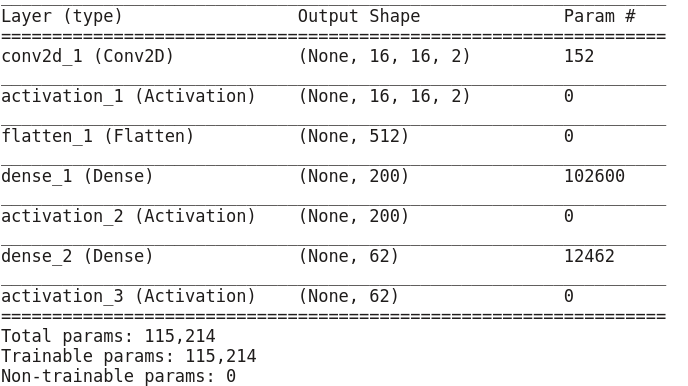
\includegraphics[scale=0.6]{SummaryCNN1}
	\caption{Zusammenfassung der Architektur für das Modell CNN1}
	\label{pic:summary-cnn1}
\end{figure}

\subsubsection{CNN2}
Das zweite CNN ist schon deutlich komplexer, als der erste Versuch. Das Eingabebild durchläuft zweimal eine Sequenz aus zweimaliger Faltung, MaxPooling und einem relativ hohen Dropout, bei dem ein Viertel der Neuronen des Pooling Layers ausgeschaltet werden. Beide Sequenzen unterscheiden sich nur durch den Parameter \texttt{filters}, der einmal auf 32 und einmal auf 64 gesetzt wurde (Listing \ref{lst:cnn2}, Zeile 3/6 und 11/13). Als Aktivierungsfunktion wurde in beide Fällen \texttt{relu} verwendet (Zeile 5, 7, 12, 14).
Die Architektur des  Netzes wird wieder durch Flattening und zwei Fully Connected Layer abgeschlossen. Im Unterschied zum vorherigen Modell enthält der der erste Fully Connected Layer deutlich mehr Neuronen und es gibt zwischen diesem und der Ausgabeschicht einen Dropout von 50\%. Wie auch zuvor wurde für den ersten Fully Connected Layer \texttt{relu} als Aktivierungsfunktion verwendet, während in der Ausgabeschicht \texttt{softmax} genutzt wird (Zeile 18 - 23). Wieder im Kontrast zur ersten Implementierung wird in dieser \texttt{rmsprop} als Optimizer genutzt (Zeile 34). Abbildung \ref{pic:summary-cnn2} stellt die Architektur des Netzes noch einmal dar.

\begin{listing} [H]
	\caption{Implementierung CNN2}
	\label{lst:cnn2}
	\begin{minted}[frame=lines, framesep=2mm, fontsize=\footnotesize, linenos]{python}
def cnn_model_2():
  model = Sequential()
  model.add(Conv2D(32, kernel_size=(3, 3), padding='same',
            input_shape=input_shape))
  model.add(Activation('relu'))
  model.add(Conv2D(32, kernel_size=(3, 3)))
  model.add(Activation('relu'))
  model.add(MaxPooling2D(pool_size=(2, 2)))
  model.add(Dropout(0.25))

  model.add(Conv2D(64, kernel_size=(3, 3), padding='same'))
  model.add(Activation('relu'))
  model.add(Conv2D(64, kernel_size=(3, 3)))
  model.add(Activation('relu'))
  model.add(MaxPooling2D(pool_size=(2, 2)))
  model.add(Dropout(0.25))

  model.add(Flatten())
  model.add(Dense(512))
  model.add(Activation('relu'))
  model.add(Dropout(0.5))
  model.add(Dense(num_classes))
  model.add(Activation('softmax'))

  opt = keras.optimizers.rmsprop(lr=0.0001, decay=1e-6)
  model.compile(loss='categorical_crossentropy', 
                optimizer=opt,
                metrics=['accuracy'])

  return model
	\end{minted}
\end{listing} 

\begin{figure} [H]
	\centering
	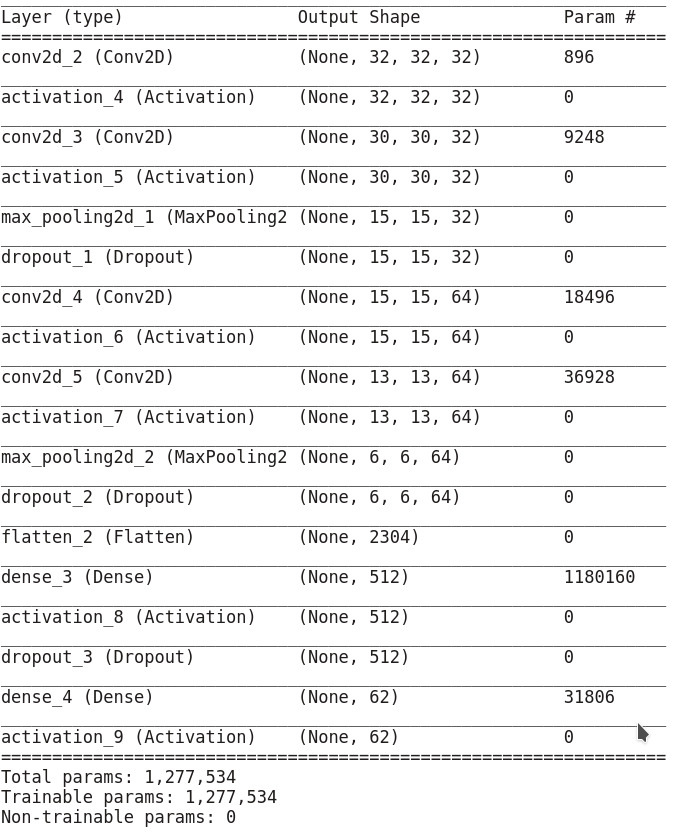
\includegraphics[scale=0.6]{SummaryCNN2}
	\caption{Zusammenfassung der Architektur für das Modell CNN2}
	\label{pic:summary-cnn2}
\end{figure}

\subsubsection{CNN3}
Die dritte Implementierung unterscheidet sich nur durch die Anzahl der Layer und Änderungen weniger Parameter von der vorherigen Implementierung. Eine weitere Sequenz von zwei Convolution, einem MaxPooling und einem Dropout Layer wurde neben einer weiteren Fully Connected Schicht eingefügt (siehe Listing \ref{lst:cnn3} und Abbildung \ref{pic:summary-cnn3}). Die Idee hinter diesem Modell war es vor allem zu untersuchen, wie sich die Qualität des Netzes durch weitere Layer und Änderungen der Parameter verhält. Leider ist es schwierig dies im Rahmen einer schriftlichen Ausarbeitung zu dokumentieren. Auch die Git-History enthält nicht alle Versuchsschritte, gibt aber einen kleinen Einblick in diese. 

\begin{listing} [H] 
	\caption{Implementierung CNN3}
	\label{lst:cnn3}
	\begin{minted}[frame=lines, framesep=2mm, fontsize=\footnotesize, linenos]{python}
def cnn_model_3():
  model = Sequential()
  model.add(Conv2D(16, kernel_size=(3, 3), padding='same',
            input_shape=input_shape))
  model.add(Activation('relu'))
  model.add(Conv2D(16, kernel_size=(3, 3)))
  model.add(Activation('relu'))
  model.add(MaxPooling2D(pool_size=(2, 2)))
  model.add(Dropout(0.125))

  model.add(Conv2D(32, kernel_size=(3, 3), padding='same'))
  model.add(Activation('relu'))
  model.add(Conv2D(32, kernel_size=(3, 3)))
  model.add(Activation('relu'))
  model.add(MaxPooling2D(pool_size=(2, 2)))
  model.add(Dropout(0.125))

  model.add(Conv2D(64, kernel_size=(3, 3), padding='same'))
  model.add(Activation('relu'))
  model.add(Conv2D(64, kernel_size=(3, 3)))
  model.add(Activation('relu'))
  model.add(MaxPooling2D(pool_size=(2, 2)))
  model.add(Dropout(0.125))

  model.add(Flatten())
  model.add(Dense(1024))
  model.add(Activation('relu'))
  model.add(Dense(512))
  model.add(Activation('relu'))
  model.add(Dropout(0.4))
  model.add(Dense(num_classes))
  model.add(Activation('softmax'))

  opt = keras.optimizers.rmsprop(lr=0.0001, decay=1e-6)
  model.compile(loss='categorical_crossentropy',
                optimizer=opt,
                metrics=['accuracy'])

  return model	
	\end{minted}
\end{listing} 

\begin{figure} [H]
	\centering
	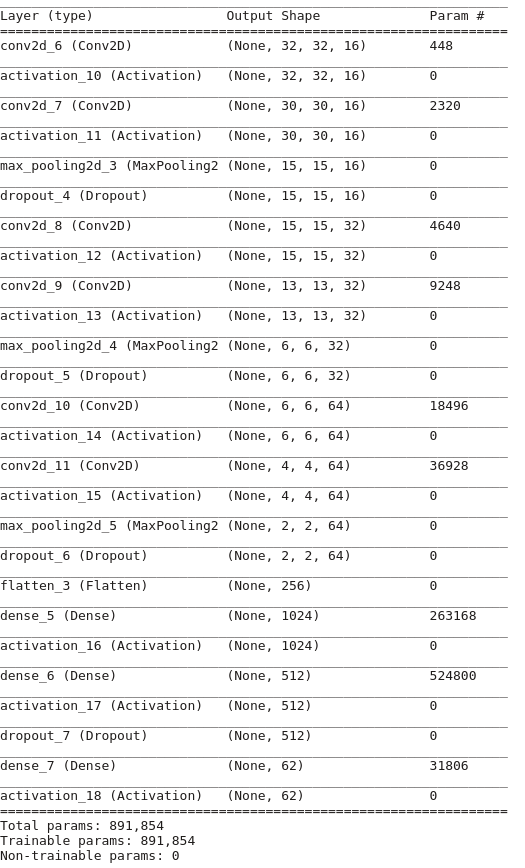
\includegraphics[scale=0.7]{SummaryCNN3}
	\caption{Zusammenfassung der Architektur für das Modell CNN3}
	\label{pic:summary-cnn3}
\end{figure}

\subsubsection{LeNet}
Um eine Referenzwert für die Güte der Modelle abseits der in TensorFlow vorgegebenen Basisimplementierung zu erhalten wurde als viertes Modell eine Implementierung von \textit{LeNet}, genauer \textit{LeNet-5} auf der Website \url{https://www.kaggle.com/tupini07/predicting-mnist-labels-with-a-cnn-in-keras/notebook} \cite{kaggle-lenet} gefunden. Diese Architektur wurde unter anderem ausgewählt, weil \textsc{Yann LeCun} als Begründer von Convolutional Neural Networks gilt, aber auch weil das Problem, für das sie in der Referenzimplementierung eingesetzt wurde, ähnlich zur Aufgabenstellung dieser Arbeit ist. Da das Modell dort allerdings für Keras 1 entwickelt wurde musste zusätzlich zu der Anpassung an den hier verwendeten Datensatz eine Portierung zu Keras 2 stattfinden. \\
\\
Neben der Anpassung an die Keras 2 API wurden im Vergleich zum Orginalcode aus \cite{kaggle-lenet} folgende Punkte angepasst:
\begin{itemize}
	\item Der \texttt{input\_shape} wurde von (28, 28, 1) (28 x 28 Pixel, 1 Farbkanal (Grayscale)) zu (32, 32, 3) (3 Farbkanäle (RGB)) geändert.
	\item Der letzte Fully Connected Layer, die Ausgangsschicht, wurde auf die Anzahl der unterschiedlichen Verkehrszeichen (Klassen) gesetzt.
\end{itemize} \ \\
Die letzte Anpassung ist zwingend notwendig, um das Netz für die Klassifikation der belgischen Verkehrszeichen zu adaptieren. Die Formatierung der Eingangsdaten wurde schon beim Laden der Daten anders festgelegt und sollte, um vergleichbare Resultate zwischen den einzelnen Implementierungen zu erreichen, konstant gehalten werden. \\
\\
Auch \textit{LeNet} ähnelt den vorhergegangenen Architekturen bis auf die Wahl der Parameter und der Anzahl der Layer. Details können Listing \ref{lst:lenet} und Abbildung \ref{pic:summary-lenet} entnommen werden.

\begin{listing} [H]
	\caption{Implementierung LeNet}
	\label{lst:lenet}
	\begin{minted}[frame=lines, framesep=2mm, fontsize=\footnotesize, linenos]{python}
def cnn_model_lenet():
  model = Sequential()

  model.add(Conv2D(6, kernel_size=(5, 5), input_shape=input_shape,
            use_bias=True,padding="same"))
  model.add(Activation('relu'))
  model.add(MaxPooling2D(pool_size=(2, 2), strides=(2, 2), padding="same"))
  model.add(Dropout(rate=0.12))

  model.add(Conv2D(16, kernel_size=(5, 5), use_bias=True, padding="same"))
  model.add(Activation('relu'))
  model.add(MaxPooling2D(pool_size=(2, 2), strides=(2, 2), padding="same"))

  model.add(Conv2D(35, kernel_size=(5, 5), use_bias=True, padding="same"))
  model.add(Activation('relu'))
  model.add(MaxPooling2D(pool_size=(2, 2), strides=(2, 2), padding="same"))

  model.add(Flatten())
  model.add(Dense(120, use_bias=True))
  model.add(Activation('relu'))
  model.add(Dropout(rate=0.5))
  model.add(Dense(84, use_bias=True))
  model.add(Activation('relu'))
  model.add(Dense(num_classes, use_bias=True))
  model.add(Activation('softmax'))

  model.compile(optimizer=Adam(lr=0.001),
                loss="categorical_crossentropy",
                metrics=['accuracy'])

  return model	
	\end{minted}
\end{listing} 

\begin{figure} [H]
	\centering
	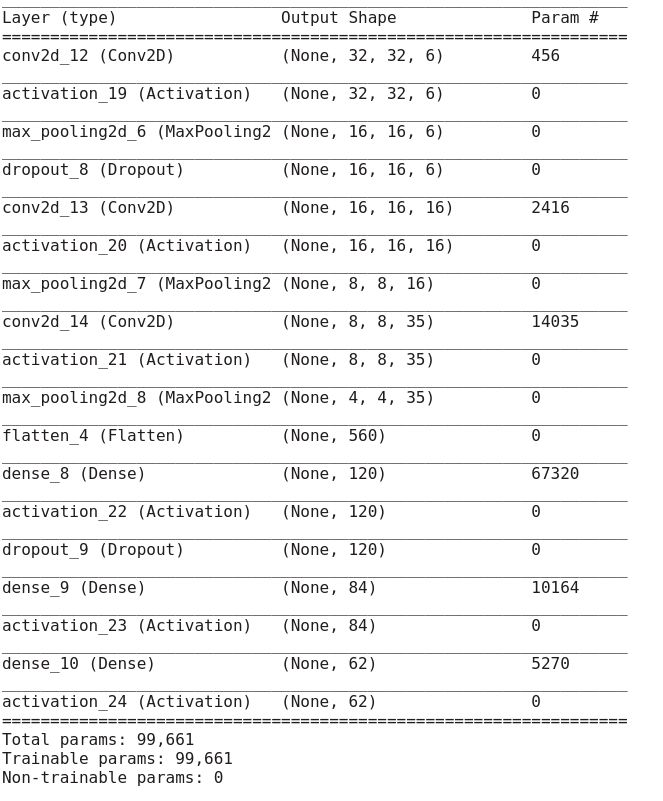
\includegraphics[scale=0.6]{SummaryLeNet}
	\caption{Zusammenfassung der Architektur für das Modell LeNet}
	\label{pic:summary-lenet}
\end{figure}

\section{Training der Modelle}
Dass für das Einlesen der Bilddaten der \texttt{ImageDataGenerator} verwendet wurde, macht sich auch beim Training der Modelle bezahlt.
Auf den Modellen kann die Methode \texttt{fit\_generator} (Listing \ref{lst:training}, Zeile 5) aufgerufen werden, die ein Batch-basiertes Training auf Basis der \texttt{DirectoryIterator} Objekte anstößt, die von der Methode \texttt{setup\_data} aus Listing \ref{lst:load-data} zurückgegeben wurden. Der Generator selbst läuft parallel zum Training, um die Erweiterung des Datensatzes in Echtzeit zu realisieren.
Der \texttt{fit\_generator} nimmt dabei zum einen den \texttt{DirectoryIterator} der Trainingsbilder (\texttt{\_train\_generator}) als Argument, aber auch den der Validierierungsdaten (\texttt{\_val\_generator}). Dies bedeutet aber nicht, dass das Modell mit den Validierungsdaten trainiert wird, sondern, dass zum Abschluss jeder Epoche, also jedes Trainingsschritts, das bisherige Modell einmal an den Validierungsdaten getestet wird. Dabei handelt es sich um einen optionalen Schritt, der keine Auswirkung auf das Modell selbst hat.
Bei den Argumenten \texttt{steps\_per\_epoch} und \texttt{validation\_steps} wurde der Wert entsprechend der Empfehlung der Keras API auf die Anzahl der Bilddateien des jeweiligen Datensatzes geteilt durch die Größe eines Batches gesetzt. Der Wert für die Anzahl der Epochen wird beim Aufruf des Trainings übergeben und hier willkürlich auf 50 gesetzt (siehe Listing \ref{lst:start-training}).

\begin{listing} [ht]
	\caption{Training und Auswertung der Modelle}
	\label{lst:training}
	\begin{minted}[frame=lines, framesep=2mm, fontsize=\footnotesize, linenos]{python}
def train_test_evaluate(_model, _train_generator, _val_generator,
				_nb_train_samples, _nb_val_samples,
				_batch_size, _epochs, _model_name):
	
  _hist = _model.fit_generator(_train_generator,
                               steps_per_epoch=_nb_train_samples // _batch_size,
                               epochs=_epochs,
                               validation_data=_val_generator,
                               validation_steps=_nb_val_samples // _batch_size)
	
  _score = _model.evaluate_generator(_val_generator, _nb_val_samples)
  print("Score for model: Test loss: ", _score[0])
  print("Score for model: Test accuracy: ", _score[1])
	
  _model.summary()
  plot_loss_accuracy(_hist, _epochs, _model_name)
  _model.save("./models/" + _model_name + ".h5")
	
  return _model, _hist, _score
	\end{minted}
\end{listing} \ \\
%
Die Methode \texttt{fit\_generator} liefert als Rückgabewert ein \texttt{History} Objekt, dass die Metriken des Trainings und der Validierung für jede Epoche enthält. Dies wird genutzt, um die Resultate für jedes Modell grafisch darzustellen \ref{lst:training}, Zeile 16. Die Implementierung der Funktion kann im beiliegenden Quellcode nachvollzogen werden. \\
\\
Analog zur Trainingsmethode \texttt{fit\_generator} wird zur Validierung des Modells die Methode \texttt{evaluate\_generator} verwendet. Diese evaluiert das fertig trainierte Modell wie es schon als Teil des Trainings für jede Epoche geschehen ist. Zurückgegeben wird ein Score bestehend aus \textit{loss} und \textit{accuracy} des Modells. \\ 
\\
Abschließend werden weitere Informationen zum Modell geloggt. Mit der Methode \texttt{summary} aus Listing \ref{lst:training}, Zeile 15 wird eine Überblick über die Architektur des Modells und die einzelnen Layer sowie deren Parameter ausgegeben. Wie schon erwähnt werden die Trainings- und Validierungsergebnisse grafisch aufbereitet und wie auch das Modell selbst gespeichert (Zeile 17). Ein trainiertes Modell kann einfach gespeichert werden, sodass es ohne erneutes Training z.B. in einer Anwendung eingesetzt werden kann. \\
\\
Das folgende Listing \ref{lst:start-training} zeigt einen Ausschnitt aus der Main-Funktion des Programms, mit dem die Daten vorbereitet und das Training, exemplarisch für das erste Modell, gestartet wird. Die genutzten Parameter \texttt{epochs} und \texttt{batch\_size} sind dabei willkürlich, aber in sinnvollen Grenzen, gewählt.

\begin{listing} [ht]
	\caption{Starten des Trainings exemplarisch für das erste Modell}
	\label{lst:start-training}
	\begin{minted}[frame=lines, framesep=2mm, fontsize=\footnotesize, linenos]{python}
if __name__ == '__main__':
  nb_train_samples = 4575
  nb_validation_samples = 2520
  epochs = 50
  batch_size = 16

  train_gen, val_gen = setup_data()

  model_cnn_1 = cnn_model_1()
  m1_model, m1_hist, m1_score = train_test_evaluate(model_cnn_1, train_gen,
                                                    val_gen, nb_train_samples,
                                                    nb_validation_samples,
                                                    batch_size, epochs, "CNN1")
	\end{minted}
\end{listing} \ \\

\section{Auswertung der Trainingsergebnisse}
Ein Blick auf die Ergebnisse aus Training und Validierung in Tabelle \ref{tab:ergebnisse} zeigt eine Schwierigkeit im maschinellen Lernen: Die Ergebnisse liegen teils sehr dicht beisammen. In den ausgeführten Trainingsläufen konnte auch kein klar favorisiertes Modell ausgemacht werden. Meist hatte zwar das Modell \textit{CNN2} um wenige Prozent das beste Ergebnis, aber auch \textit{CNN3} führte in wenigen Tests mit ein bis zwei  VorsProzentprung. \textit{LeNet} war in fast allen Durchläufen schlechter als \textit{CNN2} und \textit{CNN3}, meist aber doch besser als \textit{CNN1}.\\
\\
Bevor die Ergebnisse weiter diskutiert werden, soll noch einmal kurz darauf eingegangen werden, welche Werte in der Tabelle \ref{tab:ergebnisse} und \ref{pic:figs} abgebildet werden.
%TODO
werte: training epoche 50 und validierung
bedeutung

\begin{table} [ht]
	\begin{tabular}{|c|cc|cc||cc|cc|}
		\hline 
		 & \multicolumn{4}{|c||}{Orginal-Datensatz} & \multicolumn{4}{|c|}{Korrigierter Datensatz} \\ 
		Netz & \multicolumn{2}{|c|}{Training} & \multicolumn{2}{|c||}{Testing} & \multicolumn{2}{|c|}{Training} & \multicolumn{2}{|c|}{Testing} \\
		  & Accuracy & Loss & Accuracy & Loss & Accuracy & Loss & Accuracy & Loss \\ \hline 
		  %
		  CNN1 & 0.966 & 0.111 & 0.913 & 0.421 & 0.968 & 0.105 & 0.903 & 0.456 \\
		  CNN2 & 0.935 & 0.230 & 0.965 & 0.137 & 0.927 & 0.244 & 0.957 & 0.167 \\
		  CNN3 & 0.918 & 0.283 & 0.948 & 0.214 & 0.925 & 0.244 & 0.930 & 0.251 \\
		  LeNet& 0.899 & 0.300 & 0.943 & 0.224 & 0.903 & 0.293 & 0.927 & 0.252 \\ \hline
		 
	\end{tabular}
	\caption{Übersicht der Trainings- und Testergebnisse} \label{tab:ergebnisse}
\end{table}

\begin{figure} [!ht]
	\centering
	\subfloat[CNN1 \label{pic:fig-cnn1}]{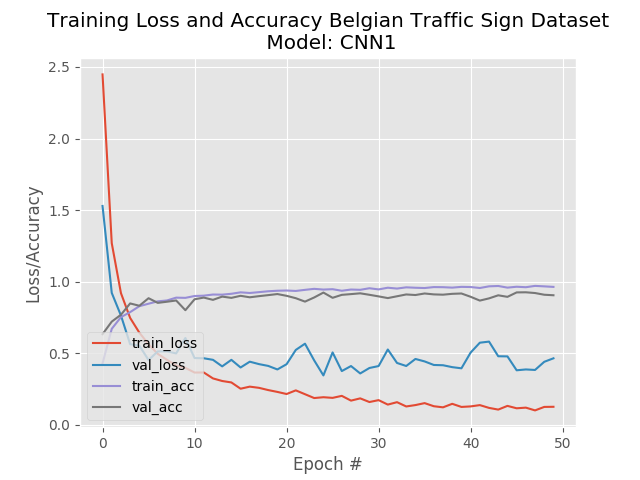
\includegraphics[scale=0.5]{CNN1}}
	\subfloat[CNN2 \label{pic:fig-cnn2}]{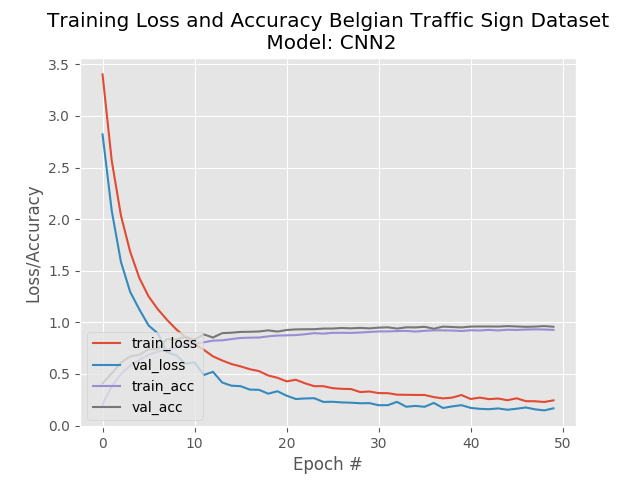
\includegraphics[scale=0.5]{CNN2}}\\
	\subfloat[CNN3 \label{pic:fig-cnn3}]{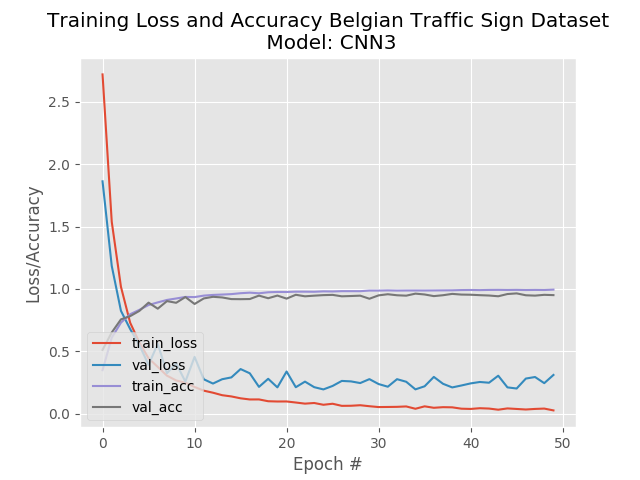
\includegraphics[scale=0.5]{CNN3}}
	\subfloat[LeNet \label{pic:fig-lenet}]{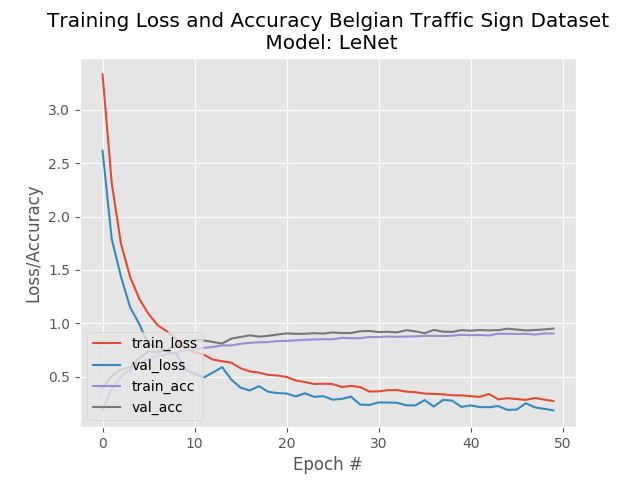
\includegraphics[scale=0.5]{LeNet}}
	\caption{Grafische Auswertung der Ergebnisse aus dem Training} \label{pic:figs}
\end{figure}


\section{Vorhersagen für unbekannte Bilder}

\section{Zusammenfassung}

